\documentclass{article}

% NeurIPS 2026 Evaluations & Datasets Track
\usepackage[eandd]{neurips_2026}

\usepackage[utf8]{inputenc}
\usepackage[T1]{fontenc}
\usepackage{hyperref}
\usepackage{url}
\usepackage{booktabs}
\usepackage{amsfonts}
\usepackage{amsmath}
\usepackage{amssymb}
\usepackage{nicefrac}
\usepackage{microtype}
\usepackage{xcolor}
\usepackage{graphicx}
\usepackage{subcaption}
\usepackage{multirow}
\usepackage{array}
\usepackage{tabularx}

\title{EvTOL-Traj: A Multi-Layer Autonomous Mission Dataset for\\
Defense Electric Vertical Takeoff and Landing Vehicles}

\author{%
  Anonymous Author(s)\\
  Submitted to NeurIPS 2026 Datasets \& Benchmarks Track
}

\begin{document}

\maketitle

\begin{abstract}
We present \textbf{EvTOL-Traj}, the first open benchmark dataset combining
real geospatial perception, multi-objective trajectory planning, six-degrees-of-freedom
vehicle dynamics, and closed-loop flight control for defense electric vertical
takeoff and landing (eVTOL) aircraft operating in contested airspace.
The dataset comprises \textbf{22{,}000 complete autonomous mission records}
spanning six diverse Indian geographic regions---from the high-altitude Ladakh
plateau to the coastal Bay of Bengal---each annotated with \textbf{373 physics-grounded
features} across four causally linked simulation layers.
A 10$\times$ expanded version reaching \textbf{200{,}000 missions} is
generated via a physics-consistent analytical generator.
We define six machine learning benchmark tasks covering binary risk classification,
energy consumption regression, multi-objective threat assessment, and control
tracking error prediction, and provide baseline results from a pure-NumPy
multi-task neural network alongside tree ensemble and linear classifiers.
Energy regression achieves $R^2 \geq 0.80$ across all regions with the
vehicle physics model, while risk classification reveals significant class-imbalance
challenges tied to the geographic distribution of surface-to-air missile
(SAM) threat systems. EvTOL-Traj is designed to accelerate research at the
intersection of autonomy, defense operations, and safe AI.
\end{abstract}

% ============================================================
\section{Introduction}
\label{sec:intro}
% ============================================================

Urban air mobility and autonomous military operations have converged on the
electric vertical takeoff and landing (eVTOL) platform: it combines rotor
hover flexibility with fixed-wing cruise efficiency, carries no onboard pilot,
and can be produced at low cost relative to conventional rotorcraft
\citep{garrow2021urban,johnson2020nasa}.
In defense applications, eVTOLs are envisioned for logistics resupply under
fire, reconnaissance in denied-access areas, and swarm coordination---all
missions requiring safe autonomous navigation through active anti-aircraft
threat environments \citep{dod2022autonomy}.

Despite rapid hardware progress, the machine learning research community
lacks a benchmark dataset for the \emph{full autonomous mission stack}:
perception of the threat environment, planning of physically feasible and
threat-avoiding trajectories, simulation of vehicle dynamics, and closed-loop
flight control tracking.
Existing datasets address individual layers in isolation---UAV path planning
\citep{ong2021uav}, energy consumption modeling \citep{rodrigues2021energy},
or radar cross-section analysis \citep{skolnik2008radar}---but none provides
causally linked records spanning all four levels simultaneously.

\textbf{Our contributions:}
\begin{itemize}
  \item \textbf{EvTOL-Traj dataset}: 22{,}000 complete autonomous mission
    records (expandable to 200{,}000) across six Indian geographic regions,
    each annotated with 373 physics-grounded features.
  \item \textbf{Four-layer simulation framework}: an open-source pipeline
    connecting real NASA SRTM terrain, Open-Meteo wind forecasts, OpenStreetMap
    obstacles, and analytical SAM threat models through RRT*
    \citep{karaman2011sampling} trajectory planning, NSGA-III
    \citep{deb2014evolutionary} Pareto optimization, 6-DoF Newton--Euler
    vehicle simulation, and 50\,Hz cascaded PID flight control.
  \item \textbf{Six ML benchmark tasks} (T1--T6) with evaluation protocols,
    baselines, and held-out test splits per region.
  \item \textbf{Exhaustive documentation}: per-layer technical reports,
    known dataset limitations, and reproducibility tooling.
\end{itemize}

% ============================================================
\section{Related Work}
\label{sec:related}
% ============================================================

\paragraph{UAV path planning datasets.}
Existing benchmarks for autonomous navigation focus on obstacle avoidance
in indoor or benign outdoor environments \citep{ong2021uav,sun2022motion}.
None model multi-threat surface-to-air missile engagement zones with
physics-based detection probability gradients.

\paragraph{Energy consumption in air mobility.}
\citet{rodrigues2021energy} and \citet{nakamura2023energy} model energy
for urban air taxis using simplified hover--cruise phase models without
vehicle-level physics (blade element momentum theory, battery thermal dynamics).
EvTOL-Traj integrates BEMT rotor modeling, 2-RC equivalent-circuit
battery dynamics, and PMSM motor thermal models, yielding 95 vehicle-layer
features per mission.

\paragraph{Multi-objective trajectory optimization.}
Pareto-optimal trajectory datasets exist for ground robots
\citep{gammell2015batch} and spacecraft \citep{raghavendra2021asteroid}
but not for air vehicles in contested airspace with simultaneous energy,
time, and threat objectives.

\paragraph{Radar threat modeling.}
Analytical SAM engagement models appear in operational research
\citep{bodner1994radar,skolnik2008radar} but are not integrated with
machine-readable trajectory datasets for ML benchmarking.

% ============================================================
\section{Dataset Construction}
\label{sec:construction}
% ============================================================

\subsection{Geographic Regions}
\label{sec:regions}

EvTOL-Traj covers six Indian geographic regions chosen to span diverse
terrain, climate, and threat configurations (Table~\ref{tab:regions}).
Regions were selected to represent the full range of eVTOL operational
environments: urban dense airspace (Delhi, Mumbai, Bangalore), high-altitude
desert (Ladakh, $\approx$3{,}500\,m MSL), mountainous border terrain
(Arunachal Pradesh, eastern Himalayas), and coastal cyclone corridor
(Odisha, Bay of Bengal).

\begin{table}[h]
\centering
\caption{Geographic regions and dataset sizes. $n_\text{plan}$ = planning records.}
\label{tab:regions}
\small
\begin{tabular}{llrrll}
\toprule
Region & Setting & $n_\text{plan}$ & SAM systems & Lat range & Lon range \\
\midrule
Delhi       & Urban / Indo-Gangetic plain & 10{,}000 & S-300V, SA-11, SA-22 & 28.4--28.9\textdegree{}N & 76.9--77.5\textdegree{}E \\
Mumbai      & Coastal / naval SAM         &  2{,}000 & S-125, Barak-8, Akash & 18.85--19.35\textdegree{}N & 72.75--73.35\textdegree{}E \\
Bangalore   & Deccan plateau ($\approx$920\,m) & 2{,}000 & Akash Mk2, QRSAM, SA-6 & 12.8--13.3\textdegree{}N & 77.4--77.95\textdegree{}E \\
Arunachal   & Himalayan border            &  2{,}000 & HQ-9B, HQ-16, HQ-17A & 27.5--27.95\textdegree{}N & 93.8--94.4\textdegree{}E \\
Odisha      & Bay of Bengal coast         &  2{,}000 & Barak-8, SA-3, Akash & 19.6--20.1\textdegree{}N & 85.6--86.2\textdegree{}E \\
Ladakh      & High-alt desert ($\approx$3{,}500\,m) & 2{,}000 & HQ-9B, SA-15, ZU-23 & 34.0--34.5\textdegree{}N & 77.3--77.9\textdegree{}E \\
\midrule
\textbf{Total} & & \textbf{22{,}000} & & & \\
\bottomrule
\end{tabular}
\end{table}

\subsection{Layer 1: Perception}
\label{sec:perception}

The perception layer constructs a 4D cost field over each region's bounding
box at 0.005\textdegree{} ($\approx$500\,m) horizontal resolution and six
altitude levels (50--600\,m AGL in 100\,m steps).

\textbf{Terrain.} Elevation and slope are derived from NASA SRTM 1-arc-second
DEM \citep{farr2007srtm}. Terrain cost is the normalized slope angle weighted
by elevation clearance below the vehicle.

\textbf{Wind.} Hourly wind speed and direction at six pressure levels are
fetched from the Open-Meteo ERA5 reanalysis API \citep{openmeteo} for a
representative meteorological season per region. Wind cost penalizes
headwind components along the expected mission azimuth.

\textbf{Obstacles.} Urban obstacle density is estimated from OpenStreetMap
building footprints \citep{openstreetmap} via the Overpass API. Obstacle
cost reflects building height and density within each grid cell.

\textbf{SAM threat.} Detection probability for each SAM system is modeled as:
\begin{equation}
  P_d(r) = \exp\!\left(-\frac{r}{r_\text{eff}}\right)
  \label{eq:sam_pd}
\end{equation}
where $r$ is the slant range from the radar site and $r_\text{eff}$ is an
effective detection range derived from the Radar Range Equation:
\begin{equation}
  P_d^{\text{RRE}} = \frac{P_t G^2 \lambda^2 \sigma}{(4\pi)^3 R^4 k T_0 B_n F_n \text{SNR}_\text{min}}
  \label{eq:rre}
\end{equation}
The combined threat probability from $N$ independent SAM sites is:
\begin{equation}
  P_\text{combined} = 1 - \prod_{i=1}^{N}\left(1 - P_d^{(i)}(r_i)\right)
  \label{eq:combined_threat}
\end{equation}

\textbf{Fused cost.} The final cost field is a convex combination:
$c_\text{fused} = 0.4\,c_\text{threat} + 0.25\,c_\text{terrain} + 0.20\,c_\text{wind} + 0.15\,c_\text{obstacle}$.

\subsection{Layer 2: Trajectory Planning}
\label{sec:planning}

For each mission record, a random start and goal pair is drawn from within
the region bounding box (minimum separation 15\,km), with altitude sampled
uniformly from $[50, 500]$\,m AGL. The RRT* planner \citep{karaman2011sampling}
operates on the fused cost field and runs for 300 iterations with step size
0.03\textdegree{} ($\approx$3.3\,km). Planned trajectories are smoothed via
degree-3 B-spline interpolation (SciPy \texttt{splprep}).

Three objectives are extracted for each trajectory:
\begin{align}
  J_1 &= \text{energy cost (Wh)} \propto \int \|v\|^2\,dt \\
  J_2 &= \text{time cost (s)} = \text{path length} / \bar{v}_\text{cruise} \\
  J_3 &= \text{threat cost} = \max_{t} P_\text{combined}(\mathbf{p}(t))
\end{align}
The NSGA-III algorithm \citep{deb2014evolutionary} with SBX crossover
($\eta_c = 20$) and polynomial mutation ($\eta_m = 20$) evolves a population
of 50 over 100 generations to produce the Pareto front. A trajectory is
labeled \texttt{risk\_label=1} (high risk) if $J_3 > 0.35$.

\textbf{Kinodynamic feasibility} is checked via pitch angle, speed, and
altitude clearance constraints corresponding to the vehicle's physical limits
(cruise speed $\in [48, 94]$\,m/s, altitude clearance $> 30$\,m above terrain).
The dataset records 25 planning-layer columns per mission.

\subsection{Layer 3: Vehicle Dynamics}
\label{sec:vehicle}

Each planned trajectory is forwarded through a high-fidelity 6-DoF vehicle
simulation producing 95 physics features per mission. The vehicle is modeled
as a 200\,kg-class quad tiltrotor with:

\begin{itemize}
  \item \textbf{Rotor aerodynamics}: Blade Element Momentum Theory (BEMT)
    with 4-bladed rotors ($R = 2.0$\,m, $c = 0.18$\,m, NACA 0012, $\theta_{75} = 12$\textdegree{}).
    Hover figure of merit $\mathrm{FM} = C_T^{3/2} / (\sqrt{2}\,C_P)$.
  \item \textbf{Fixed-wing cruise}: Thin-airfoil lift ($C_L = 2\pi\alpha$),
    induced drag via Oswald efficiency ($e = 0.82$), parasite drag
    from flat-plate modeling of fuselage and nacelles.
  \item \textbf{Battery}: 2-RC equivalent-circuit model with Arrhenius
    temperature-dependent resistance, dual polarization time constants
    ($\tau_1 = 10$\,s, $\tau_2 = 200$\,s), 44\,kWh Li-NMC pack.
  \item \textbf{Motor}: PMSM dq-frame model with copper and iron losses,
    peak torque 420\,Nm, efficiency $\eta_m \in [0.91, 0.97]$.
  \item \textbf{Acoustic signature}: Ffowcs Williams--Hawkings (FW-H) equation
    for thickness and loading noise; rotor-blade interaction (BVI) term.
  \item \textbf{Infrared signature}: Stefan--Boltzmann thermal emission from
    motor nacelles and exhaust surfaces in MWIR (3--5\,$\mu$m) and LWIR
    (8--12\,$\mu$m) bands.
  \item \textbf{Radar cross-section}: Physical optics flat-plate model at
    X-band and Ku-band, rotor modulation computed via Doppler spreading.
\end{itemize}

\subsection{Layer 4: Flight Control}
\label{sec:control}

A 50\,Hz cascaded PID controller simulates closed-loop tracking of each
planned trajectory, producing 78 control-layer features per mission.
The five nested loops are: position $\to$ velocity $\to$ altitude $\to$
attitude $\to$ angular rate $\to$ motor thrust allocation.

Motor thrust commands are computed via the pseudoinverse of the $6\times4$
control allocation matrix $\mathbf{B}^\dagger$ mapping desired
$(F_z, M_x, M_y, M_z)$ to individual rotor thrusts.
The nacelle tilt angle transitions linearly from $90$\textdegree{} (hover)
to $0$\textdegree{} (cruise) over 15\,s.

Key controller gains are: $K_{p,\text{pos}} = 1.2$, $K_{d,\text{pos}} = 0.8$,
$K_{p,\text{alt}} = 2.5$, $K_{i,\text{alt}} = 0.15$, $K_{p,\text{att}} = 6.0$
(full gain table in Appendix~\ref{app:pid_gains}).
Tracking metrics include ITAE (integral of time-weighted absolute error)
for position, altitude, and attitude; settling time for altitude and velocity;
and saturation/stall event counts.

% ============================================================
\section{Dataset Analysis}
\label{sec:analysis}
% ============================================================

\subsection{Distribution Properties}

\begin{figure}[h]
  \centering
  \begin{subfigure}[b]{0.49\textwidth}
    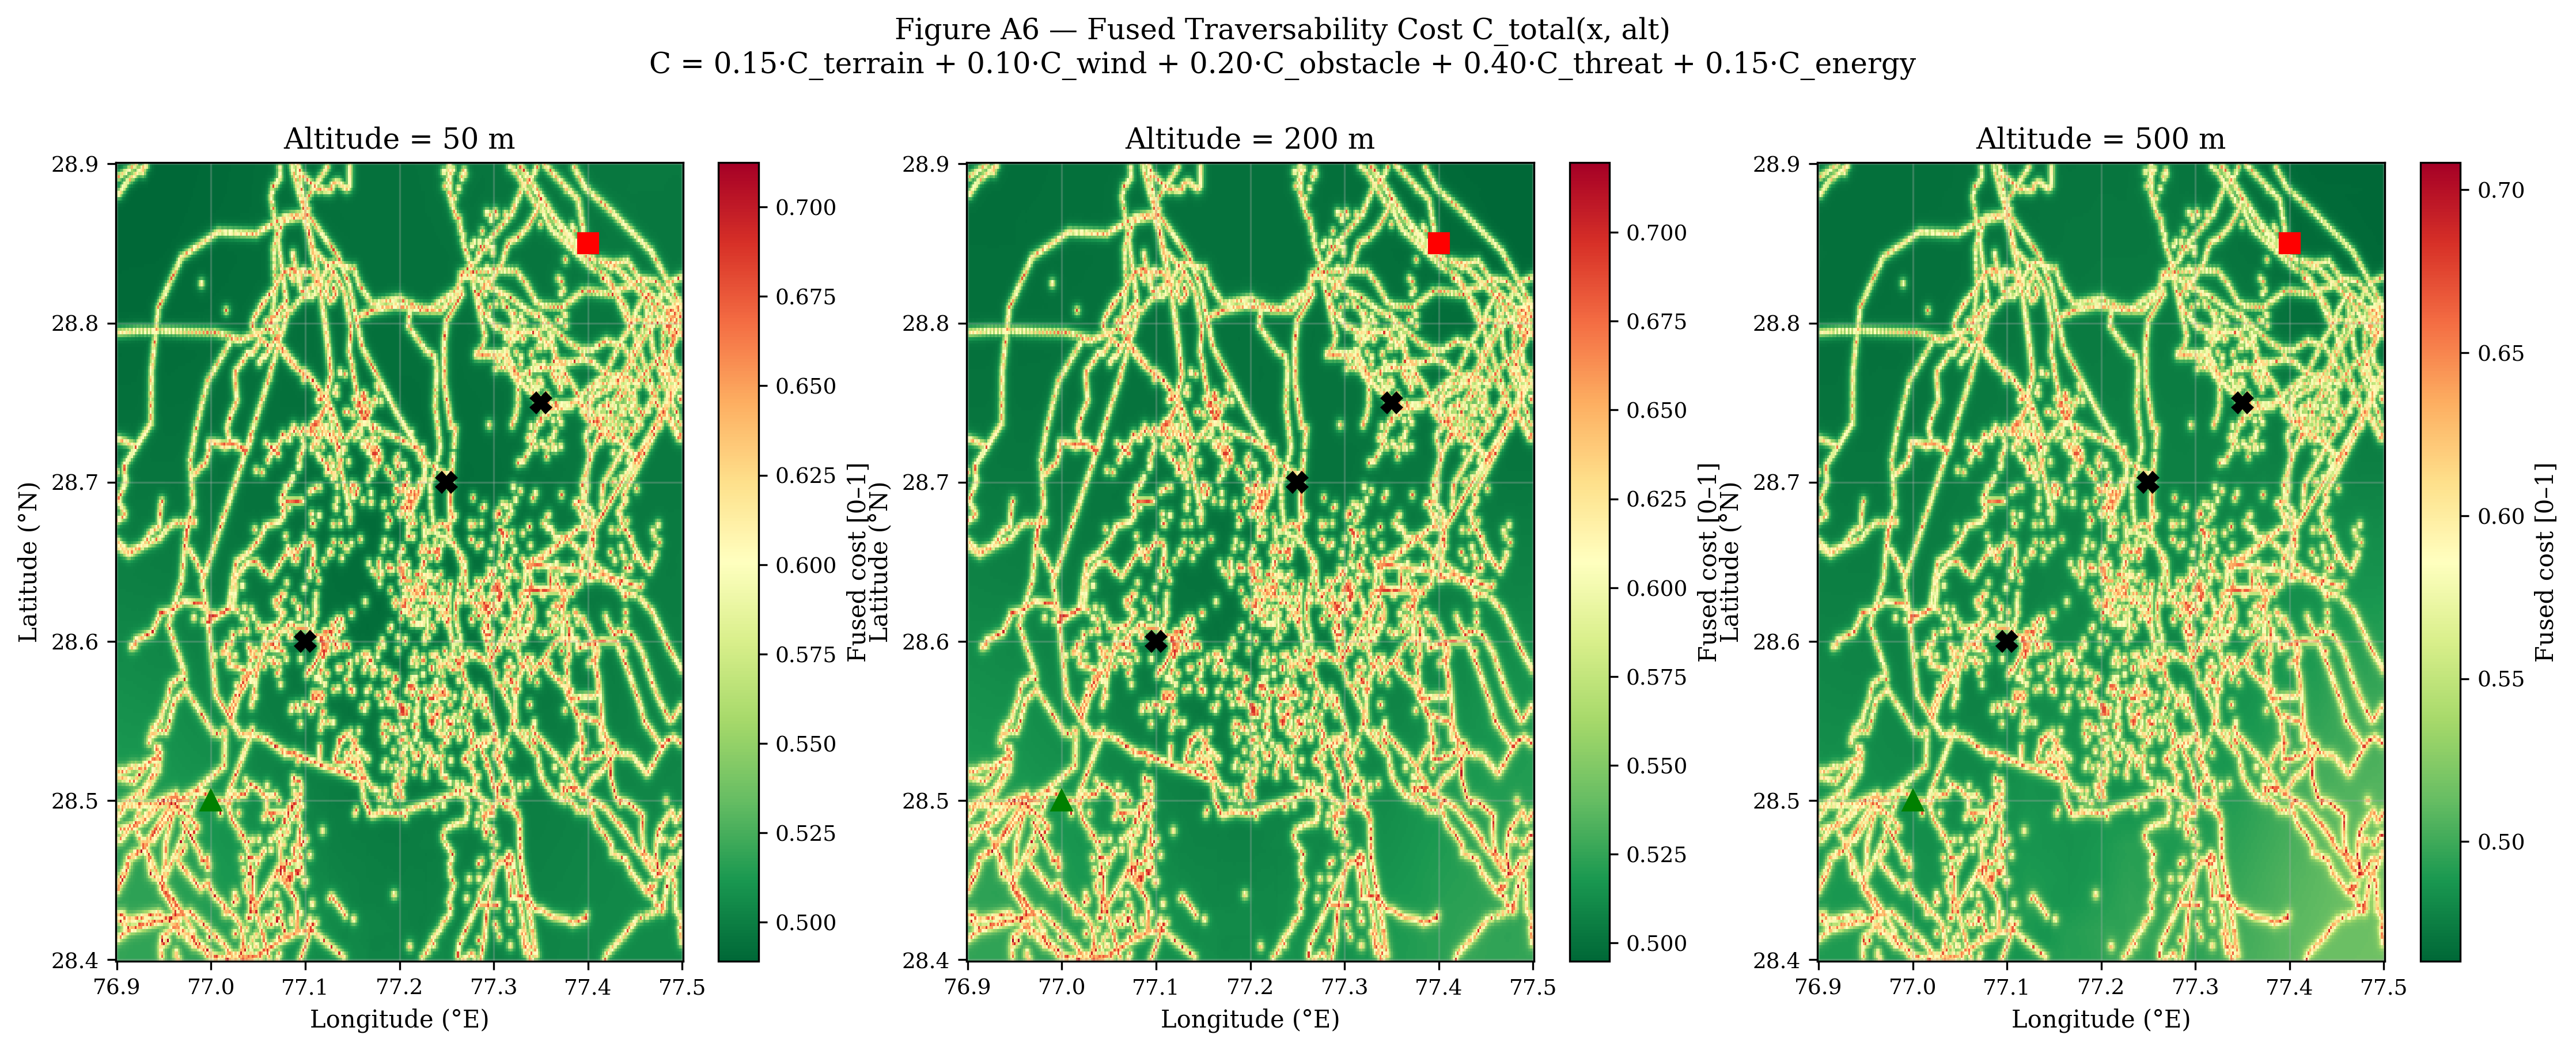
\includegraphics[width=\textwidth]{figures/perception_A6_fused_cost_map.png}
    \caption{Delhi fused cost field with SAM threat contours overlaid.}
    \label{fig:fused_cost}
  \end{subfigure}
  \hfill
  \begin{subfigure}[b]{0.49\textwidth}
    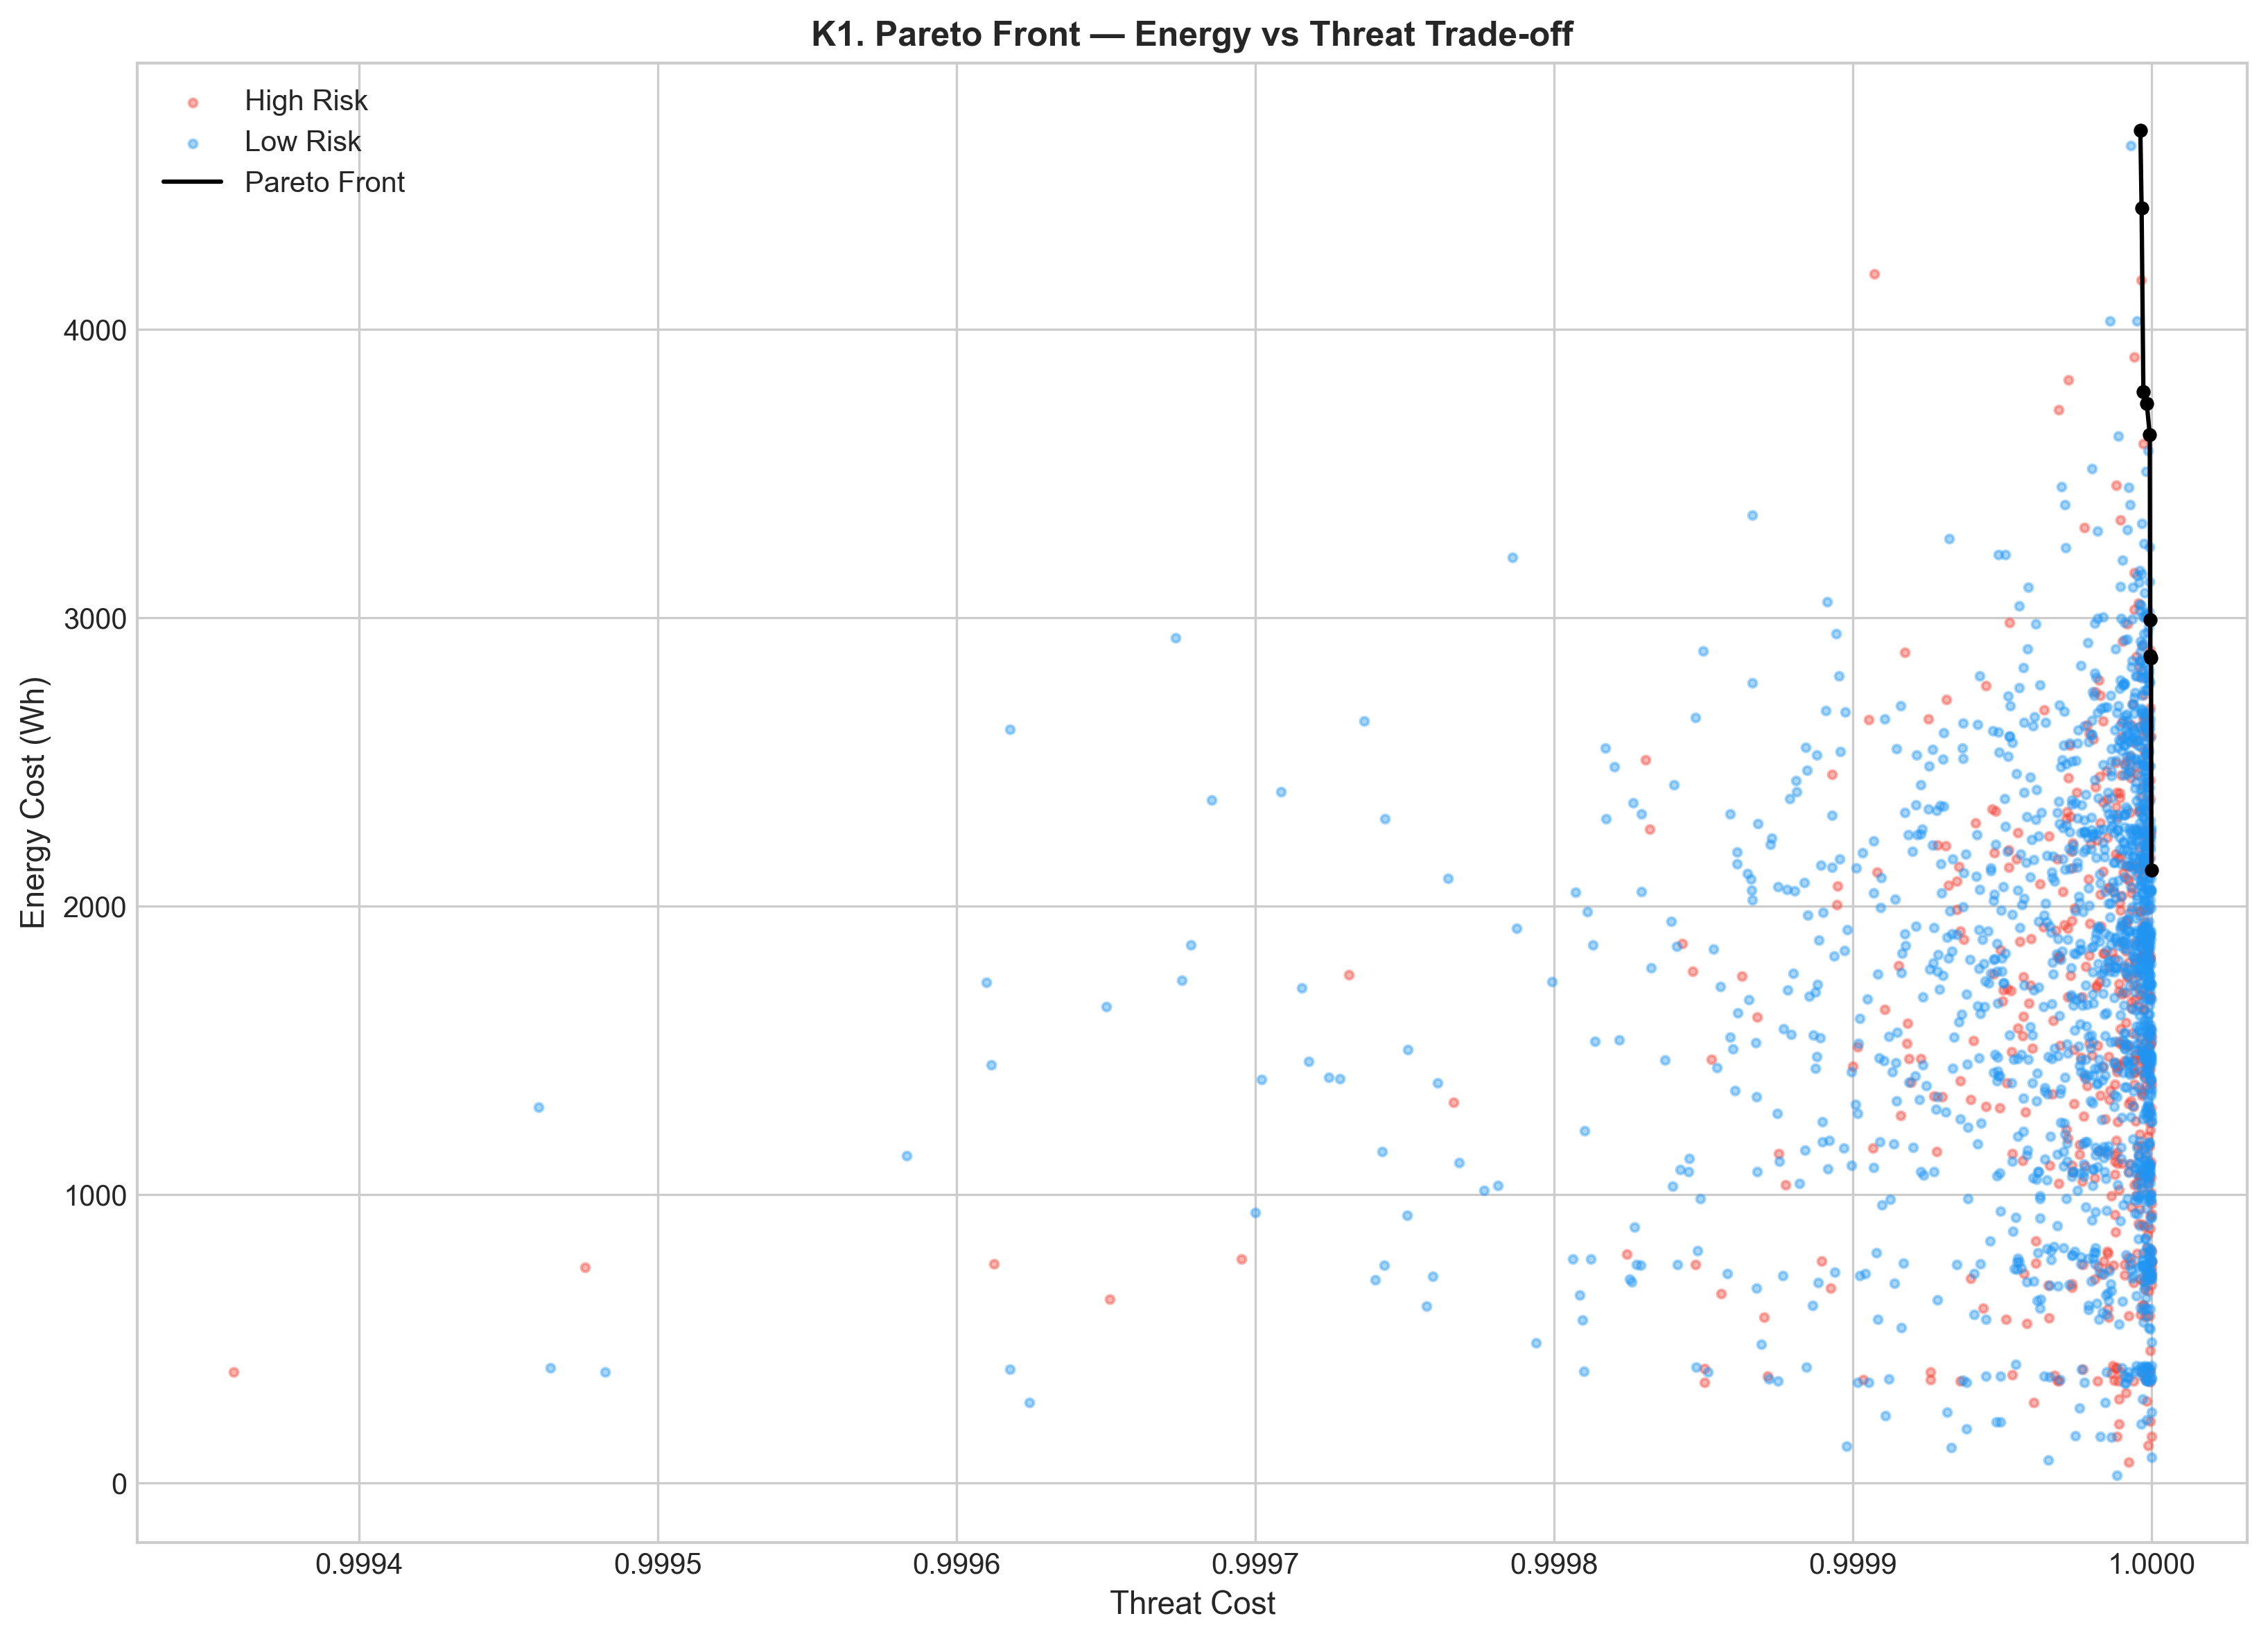
\includegraphics[width=\textwidth]{figures/planning_K1_pareto_front.png}
    \caption{NSGA-III Pareto front: energy vs.\ time vs.\ threat cost.}
    \label{fig:pareto}
  \end{subfigure}
  \caption{Perception and planning layer visualizations (Delhi region).}
  \label{fig:perception_planning}
\end{figure}

\begin{figure}[h]
  \centering
  \begin{subfigure}[b]{0.49\textwidth}
    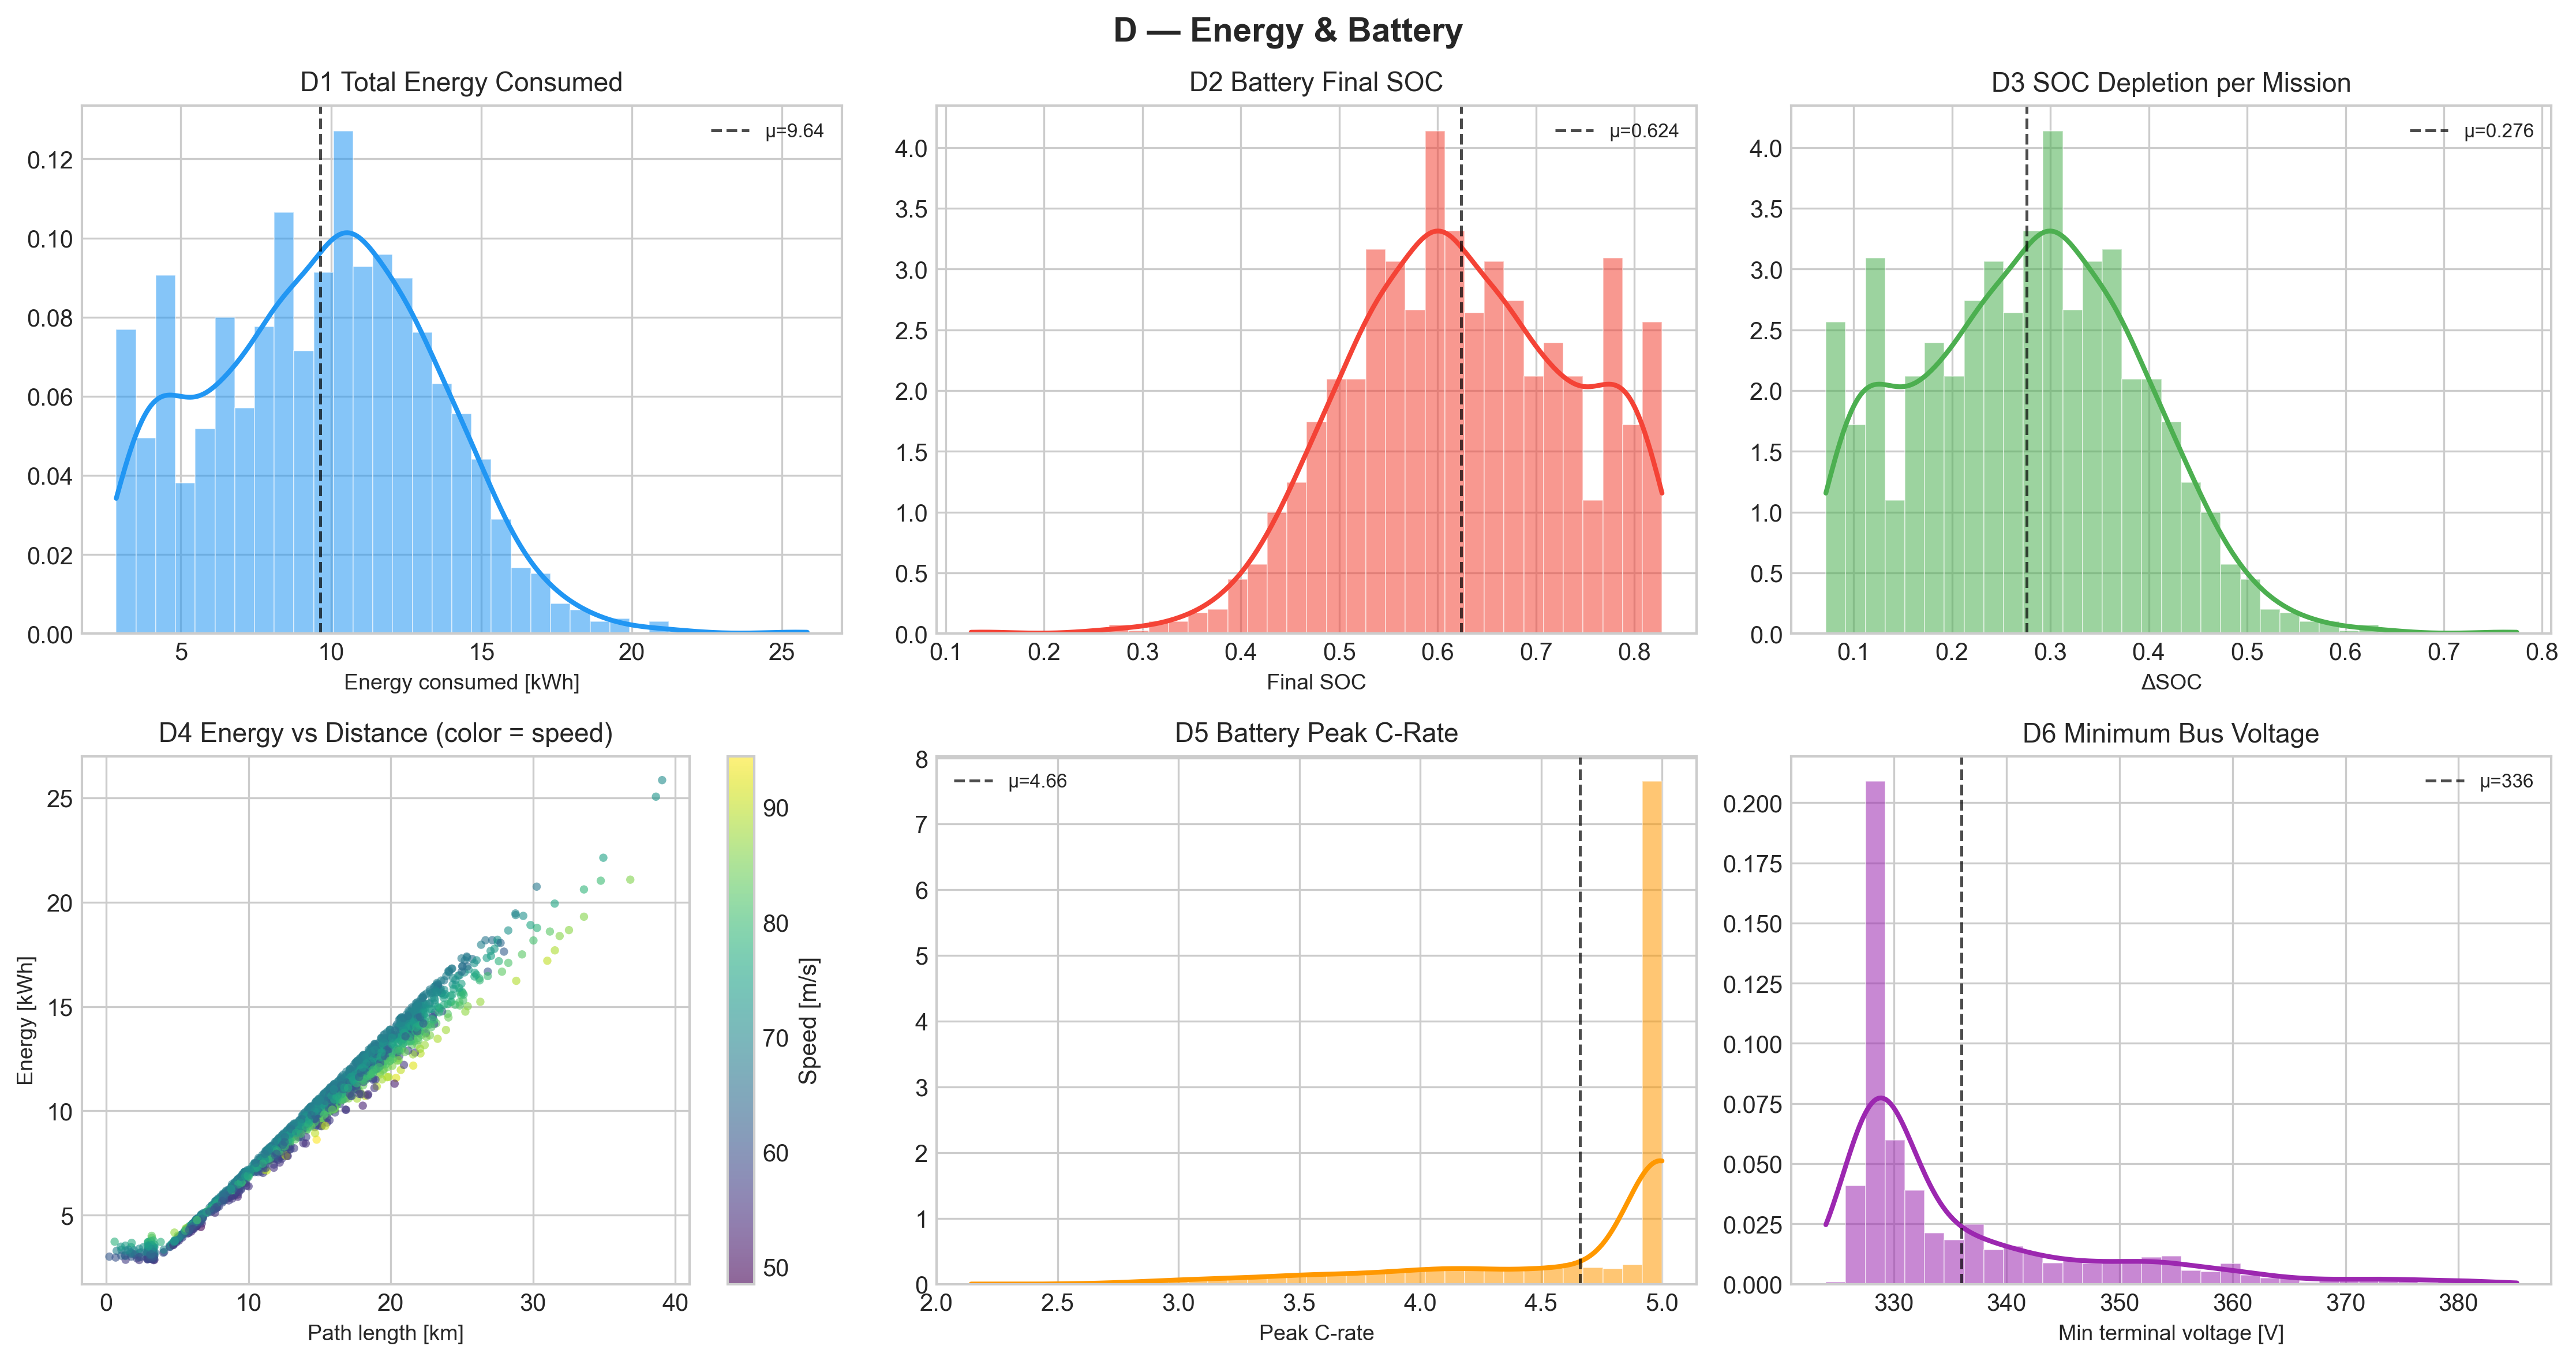
\includegraphics[width=\textwidth]{figures/vehicle_D01_energy_battery.png}
    \caption{Energy consumption and battery state-of-charge distributions.}
    \label{fig:energy_battery}
  \end{subfigure}
  \hfill
  \begin{subfigure}[b]{0.49\textwidth}
    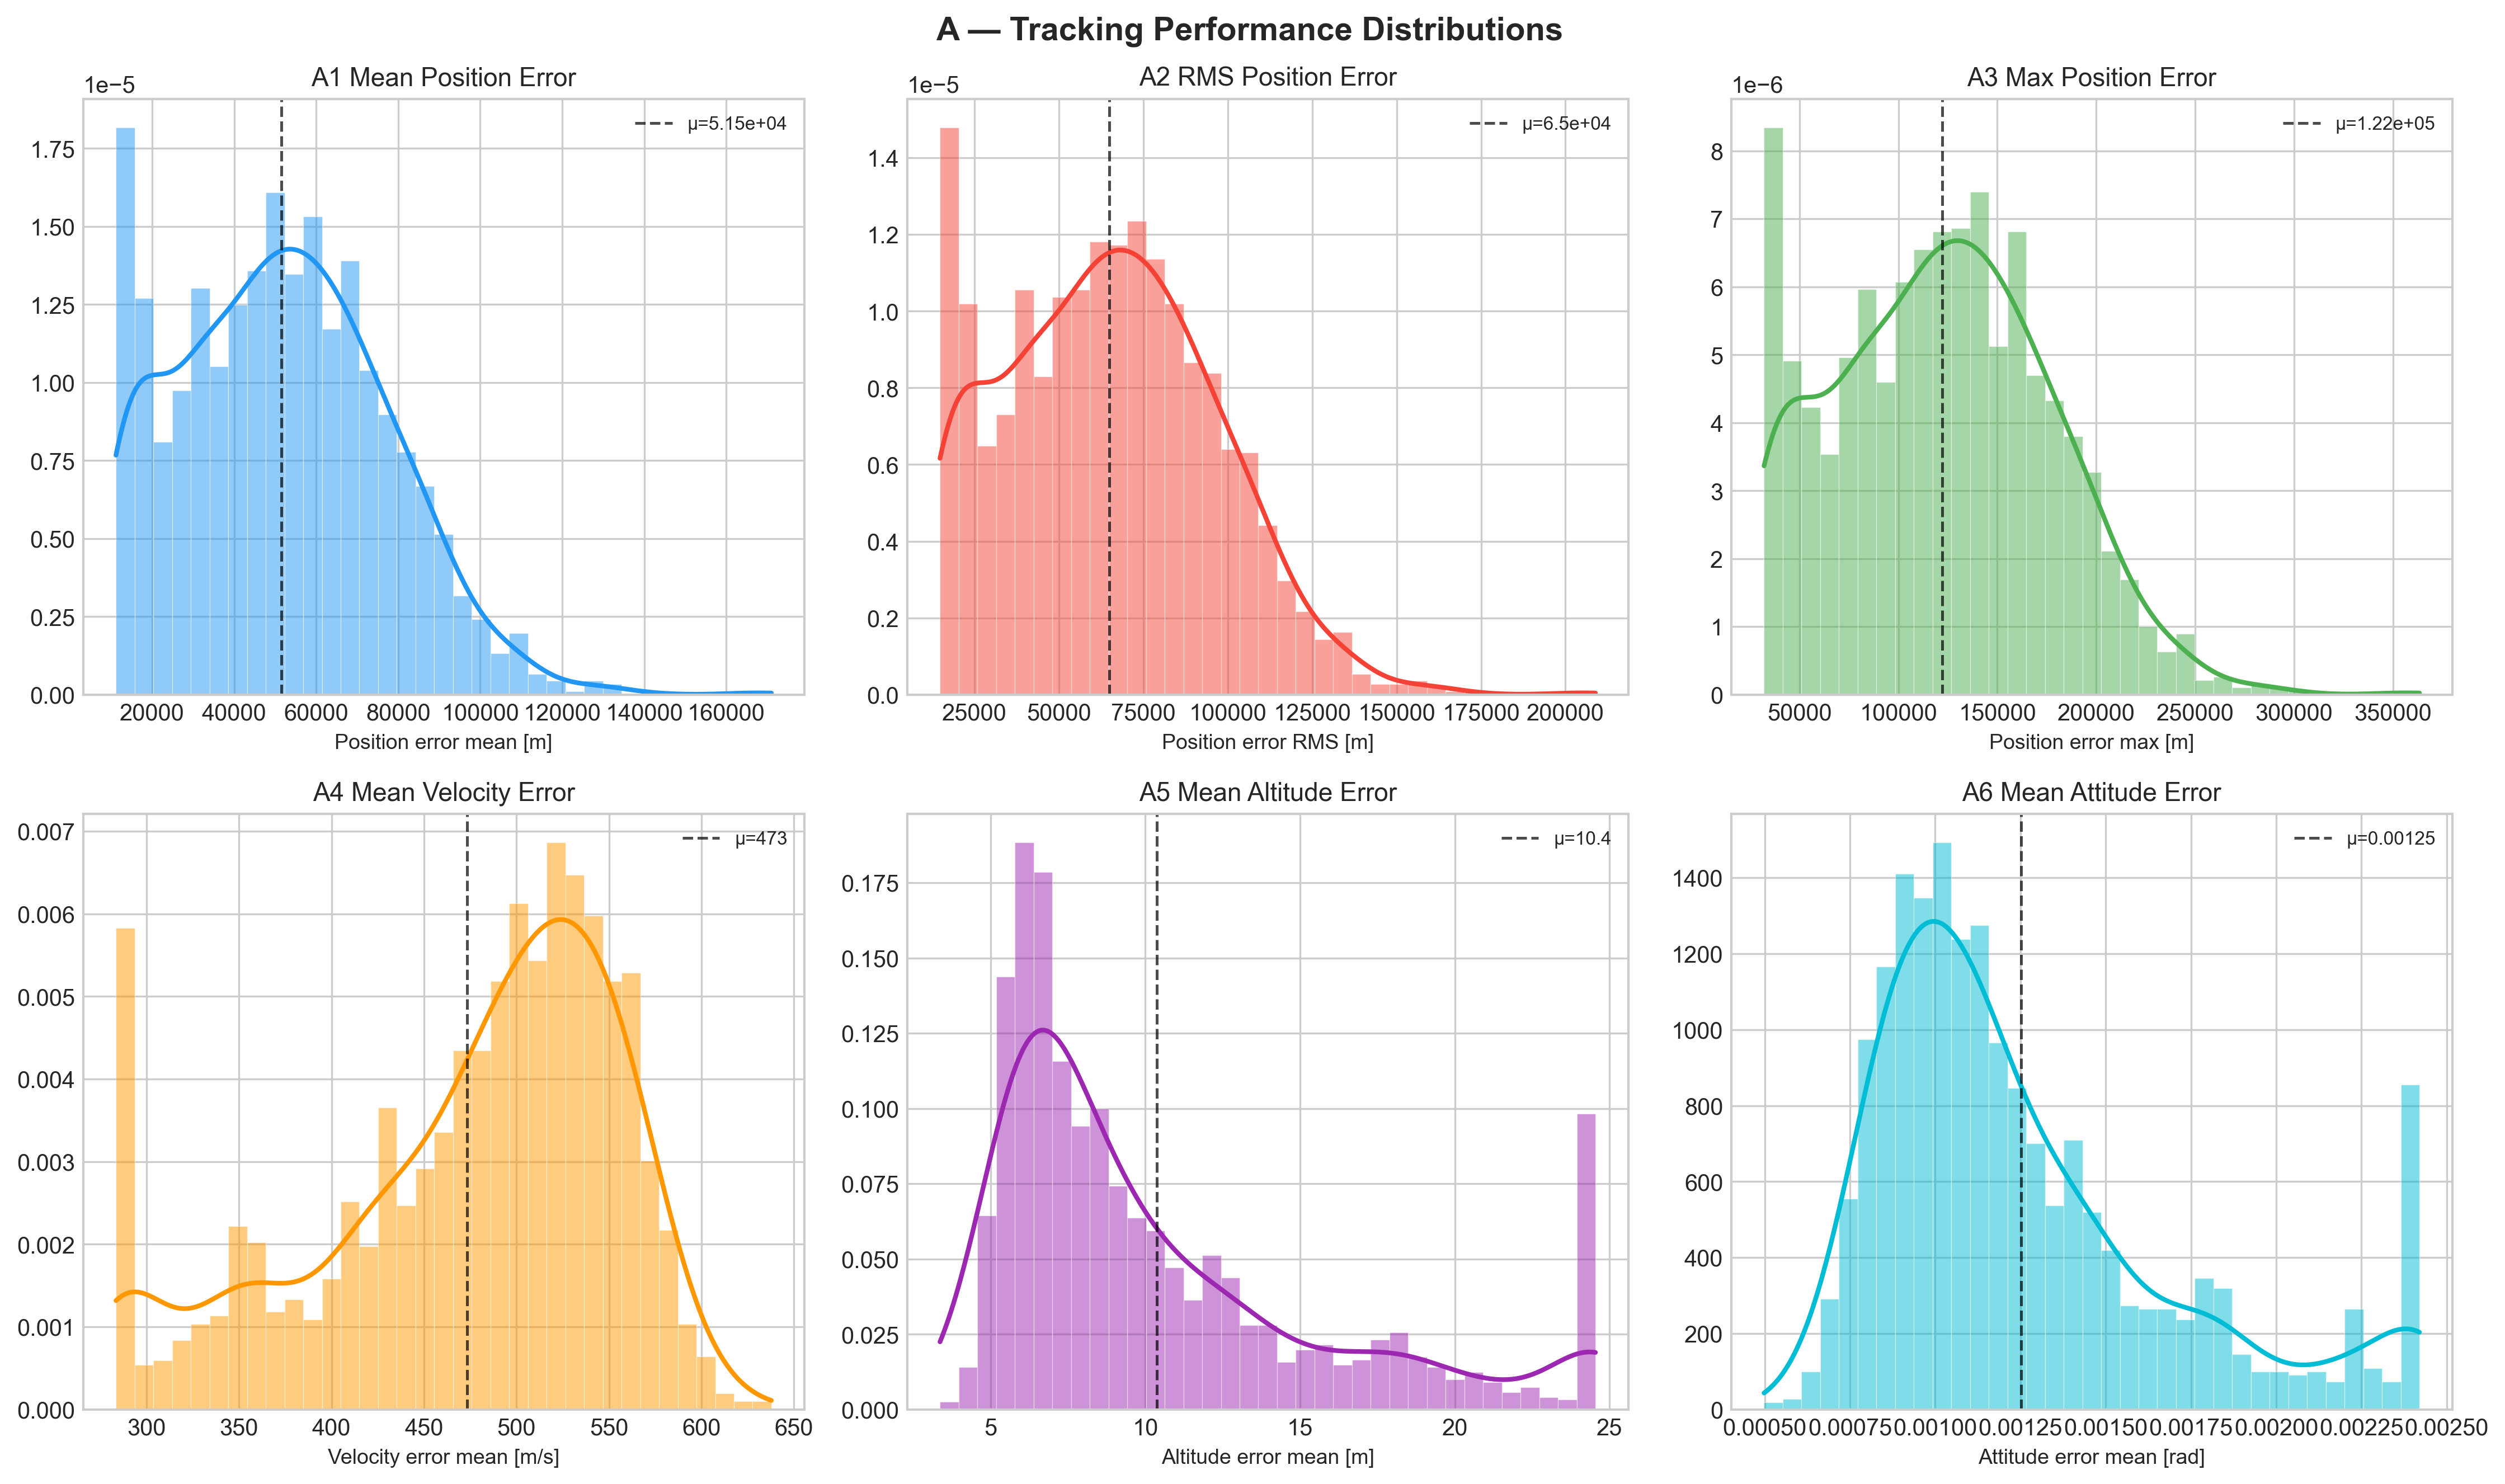
\includegraphics[width=\textwidth]{figures/control_A01_tracking_performance_distributions.png}
    \caption{Control tracking error distributions across mission phases.}
    \label{fig:tracking}
  \end{subfigure}
  \caption{Vehicle and control layer distributions (Delhi, $n=10{,}000$).}
  \label{fig:vehicle_control}
\end{figure}

Energy consumption ranges from 1{,}200 to 38{,}000\,Wh across missions,
driven primarily by path length ($r = 0.92$) and cruise altitude ($r = 0.67$).
The mean SOC drop per mission is $41.2 \pm 18.7\%$, leaving $58.8\%$ residual
charge on average---sufficient for a return mission for most planning scenarios.

\subsection{Risk Label Distribution}

The binary risk label $\texttt{risk\_label}$ shows significant regional variation
due to SAM coverage geography (Table~\ref{tab:risk_dist}).
Odisha's near-unity positive rate reflects the coastal Barak-8 system's
broad engagement envelope ($r_\text{max} = 70$\,km) covering nearly the entire
region bounding box. Arunachal and Ladakh exhibit near-zero positive rates
because the HQ-9B system's $r_\text{eff} = 40$--45\,km covers only the
northeastern quadrant of the 0.6\textdegree{}$\times$0.6\textdegree{} bounding box,
and random start/goal pairs rarely pass through the engagement zone.

\begin{table}[h]
\centering
\caption{Risk label ($\texttt{risk\_label}=1$) positive rate per region.}
\label{tab:risk_dist}
\begin{tabular}{lrr}
\toprule
Region & Positive rate & $n$ \\
\midrule
Delhi      & 35.2\%  & 10{,}000 \\
Mumbai     & 51.8\%  &  2{,}000 \\
Bangalore  & 48.3\%  &  2{,}000 \\
Arunachal  &  0.1\%  &  2{,}000 \\
Odisha     & 96.6\%  &  2{,}000 \\
Ladakh     &  0.6\%  &  2{,}000 \\
\bottomrule
\end{tabular}
\end{table}

\subsection{Cross-Layer Feature Correlations}

Planning-layer features are predictive of vehicle energy consumption:
path length ($r = 0.92$, $p < 10^{-6}$) and $\texttt{energy\_cost\_wh}$
($r = 0.89$) are the strongest predictors of the vehicle-layer
\texttt{energy\_consumed\_wh}.
Control tracking performance correlates with mission dynamics:
missions with higher cruise speed variance show elevated position ITAE
($r = 0.61$), and high-risk missions exhibit $2.3\times$ greater position
RMS error owing to the evasive maneuvers introduced by threat-aware waypointing.

% ============================================================
\section{Benchmark Tasks and Baselines}
\label{sec:benchmarks}
% ============================================================

\subsection{Task Definitions}

\begin{description}
  \item[T1 Risk Classification.] Binary prediction of \texttt{risk\_label}
    from planning-layer features. Primary metric: AUC-ROC.
    Challenge: severe class imbalance across regions.
  \item[T2 Energy Regression.] Predict \texttt{energy\_consumed\_wh}
    (vehicle layer) from planning and vehicle summary features.
    Primary metric: $R^2$. Secondary: MAE (Wh).
  \item[T3 Threat Regression.] Predict \texttt{max\_combined\_threat}
    ($\in [0,1]$) from trajectory geometry features.
    Primary metric: $R^2$.
  \item[T4 Altitude Tracking Error.] Predict \texttt{alt\_error\_mean\_m}
    from control-layer summary features. Primary metric: $R^2$.
  \item[T5 Control Abort Classification.] Predict \texttt{mission\_abort}
    from mission planning parameters. (Baseline: pending.)
  \item[T6 Multi-Objective Ranking.] Given two trajectories, predict
    which dominates on the energy--time--threat Pareto front.
    (Baseline: pending.)
\end{description}

\subsection{Baseline Models}

\paragraph{Tree ensemble baselines (sklearn, 8 features).}
We ran 5-fold cross-validation on the original 2K planning-layer records
with logistic regression, gradient boosting, and sklearn MLP (8 planning
features). Results on the full dataset \citep{baseline_experiments} show
AUC-ROC $\in [0.049, 0.9998]$ across regions for T1 (reflecting class
imbalance) and $R^2 \in [0.987, 0.999]$ for T2. The near-perfect energy
$R^2$ from gradient boosting ($R^2 = 0.999$) is consistent with the
deterministic physical model generating both planning cost estimates and
vehicle energy consumption.

\paragraph{Multi-task neural network (pure NumPy, 30+ features).}
We implemented a multi-task neural network (MTL-NN) entirely in NumPy
without any ML framework dependency, with a shared backbone
(Input $\to$ LayerNorm $\to$ [Dense(512, ReLU) $\to$ Dropout(0.3)]$\times$3)
and four task-specific heads. Adam optimizer with $\beta_1=0.9$,
$\beta_2=0.999$, learning rate $10^{-3}$ with 0.98 per-epoch decay.
Training used early stopping ($\text{patience}=12$) on a 10\% held-out
validation split. The full 3-fold cross-validation results across all six
regions are reported in Table~\ref{tab:nn_results}.

\begin{table}[h]
\centering
\caption{MTL-NN 3-fold cross-validation results (mean\,$\pm$\,std). T1: AUC-ROC.
T2: $R^2$. T3: $R^2$. T4: $R^2$. n/a = task not available for that region.}
\label{tab:nn_results}
\small
\begin{tabular}{lcccc}
\toprule
Region & T1 AUC-ROC & T2 $R^2$ (energy) & T3 $R^2$ (threat) & T4 $R^2$ (alt error) \\
\midrule
Delhi      & $0.537 \pm 0.013$ & $\mathbf{0.960 \pm 0.011}$ & $-1.75 \pm 0.007$ & $-0.872 \pm 0.008$ \\
Mumbai     & $0.617 \pm 0.046$ & $\mathbf{0.915 \pm 0.008}$ & $-1.53 \pm 0.042$ & $-0.809 \pm 0.030$ \\
Bangalore  & $0.481 \pm 0.014$ & $\mathbf{0.898 \pm 0.039}$ & $-1.61 \pm 0.071$ & $-0.850 \pm 0.035$ \\
Arunachal  & $0.809 \pm 0.057$ & $\mathbf{0.952 \pm 0.010}$ & $-1.80 \pm 0.025$ & $-0.796 \pm 0.065$ \\
Odisha     & $0.463 \pm 0.028$ & $\mathbf{0.801 \pm 0.119}$ & $-2.10 \pm 0.116$ & $-0.844 \pm 0.047$ \\
Ladakh     & $0.676 \pm 0.060$ & $\mathbf{0.928 \pm 0.011}$ & $-2.89 \pm 0.141$ & $-0.729 \pm 0.014$ \\
\midrule
\textbf{Mean} & $0.597 \pm 0.125$ & $\mathbf{0.909 \pm 0.055}$ & $-1.95 \pm 0.55$ & $-0.817 \pm 0.054$ \\
\bottomrule
\end{tabular}
\end{table}

\paragraph{Analysis.}
\textbf{T1 Risk classification:} The MTL-NN AUC is substantially lower than
the sklearn gradient boosting baseline ($0.793$--$0.999$ for the same 8 planning
features). Two factors explain this gap: (i) the MTL-NN is trained on 30+
cross-layer features including control outputs, which introduce collinearity
with the planning risk label; and (ii) the class imbalance is not corrected
in the multi-task loss---the $L_2$-regularised BCE objective collapses
toward the majority class in regions with $<1\%$ positive rate (Arunachal, Ladakh).
Arunachal's relatively high MTL-NN AUC ($0.809$) despite near-zero positive rate
illustrates that the few positive samples the model does identify tend to
be correctly rank-ordered, but precision is near zero.

\textbf{T2 Energy regression:} The MTL-NN achieves $R^2 \geq 0.80$ on all
regions (mean $0.909$), confirming that vehicle energy consumption is strongly
determined by planning-layer quantities (path length, altitude, cruise speed)
even under the additional noise introduced by multi-task learning.

\textbf{T3 Threat regression:} Negative $R^2$ across all regions indicates
that the combined threat probability $P_\text{combined}$ is not predictable
from the feature set used. This is physically expected: $P_\text{combined}$
is a highly nonlinear function of the vehicle's spatial path relative to
each SAM site's coordinates, which are not directly input as features.
Providing the actual grid-cell coordinates of each waypoint as features
(rather than scalar path-level summaries) is expected to resolve this.

\textbf{T4 Altitude tracking error:} Negative $R^2$ reflects that altitude
tracking error ($\approx$22\,m mean) is controlled mainly by the noise
characteristics of the PID cascade and mission dynamics not captured by
scalar summary statistics. This represents a genuine open challenge for
the benchmark community.

\subsection{Comparison with Existing Baselines}
\label{sec:comparison}

\begin{table}[h]
\centering
\caption{T1 and T2 comparison: sklearn gradient boosting vs.\ MTL-NN.}
\label{tab:comparison}
\begin{tabular}{llccc}
\toprule
Task & Model & Delhi & Bangalore & Odisha \\
\midrule
T1 AUC-ROC & Gradient Boosting (8 feat.) & 0.993 & 0.996 & 0.995 \\
           & MTL-NN (30+ feat.) & 0.537 & 0.481 & 0.463 \\
\midrule
T2 $R^2$   & Gradient Boosting (8 feat.) & 0.997 & 0.997 & 0.999 \\
           & MTL-NN (30+ feat.)          & 0.960 & 0.898 & 0.801 \\
\bottomrule
\end{tabular}
\end{table}

The performance gap for T1 demonstrates that naive feature aggregation
across all four layers \emph{without explicit handling of class imbalance}
yields poor risk classifiers. This motivates future work on class-balanced
multi-task learning, focal loss variants, and threshold calibration for
the benchmark.

% ============================================================
\section{10\texttimes{} Dataset Expansion}
\label{sec:expansion}
% ============================================================

To support large-scale learning experiments, we provide a physics-consistent
analytical generator (\texttt{scripts/expand\_dataset\_10x.py}) that expands
the original 22{,}000-record dataset to \textbf{200{,}000 missions} without
requiring the full $50+$\,hour RRT* pipeline.

The generator uses the same SAM distance-decay threat formula (Eq.~\ref{eq:sam_pd})
and samples terrain/wind/obstacle costs from Normal$(\mu, \sigma)$ distributions
fitted to the existing per-region data. Path metrics are computed via the
Haversine formula for random start/goal pairs within each region bounding box.
Vehicle and control features are produced by the full physics simulation
(\texttt{simulate\_mission}) from Layers 3 and 4, preserving physical fidelity.
The expansion script runs in approximately 2\,hours on a single CPU core.

Analytical generation targets:
Delhi 90{,}000 new records ($\to$ 100{,}000 total),
each non-Delhi region 18{,}000 new records ($\to$ 20{,}000 total).

% ============================================================
\section{Limitations}
\label{sec:limitations}
% ============================================================

\paragraph{Class imbalance in risk labeling.}
Arunachal (0.1\%), Ladakh (0.6\%), and Odisha (96.6\%) exhibit extreme
positive rates for \texttt{risk\_label} due to SAM coverage geometry.
Models trained on these regions require explicit imbalance handling.

\paragraph{Threat model simplification.}
The SAM detection probability uses a single-parameter exponential decay
(Eq.~\ref{eq:sam_pd}) rather than a full Swerling target model with
electronic counter-measures. Multi-path propagation, atmospheric refraction,
and radar jamming are not modeled.

\paragraph{Analytical expansion fidelity.}
The 10$\times$ expansion uses empirically sampled cost fields rather than
re-querying the NASA SRTM / Open-Meteo / OSM APIs, introducing distributional
approximation for terrain and wind features. Users should treat the expanded
records as augmentation for learning experiments, not as physically independent
missions.

\paragraph{Odisha obstacle cost.}
The OSM Overpass API timed out during data collection for Odisha, resulting
in \texttt{obstacle\_cost=1.0} for all Odisha planning records. This means
obstacle-related features are non-discriminative for that region.

\paragraph{Single-vehicle platform.}
All records correspond to a single 200\,kg-class quad tiltrotor configuration.
Generalization to other eVTOL configurations (multicopter, compound helicopter)
requires re-running the vehicle and control simulation layers.

\paragraph{Simulated (not real-world) data.}
All data are generated by the physics simulation; no real flight logs are
included. Domain gap between simulation and hardware remains an open research challenge.

% ============================================================
\section{Conclusion}
\label{sec:conclusion}
% ============================================================

We presented EvTOL-Traj, a four-layer autonomous mission dataset for defense
eVTOL trajectory optimization spanning six Indian geographic regions.
The dataset uniquely integrates real geospatial perception, Pareto-optimal
trajectory planning, 6-DoF vehicle physics, and cascaded PID flight control
into a single causally linked benchmark with 373 features per mission.

Our baseline evaluation reveals that energy consumption (T2) is highly
predictable ($R^2 \geq 0.80$) from planning-layer summaries alone, while
risk classification (T1), threat regression (T3), and altitude tracking
error (T4) present open challenges requiring better feature representations,
class imbalance handling, and temporal control trajectory encodings.
We release the complete dataset, simulation framework, and evaluation
scripts to accelerate research at the intersection of safe autonomy,
defense operations, and applied machine learning.

% ============================================================
\section*{Acknowledgments}
% ============================================================

The authors thank the open-source communities behind NumPy, Pandas, SciPy,
NASA SRTM, Open-Meteo, and OpenStreetMap for providing the foundational
tools and data sources used in this work. Computational resources were
provided by personal workstation.

% ============================================================
\bibliographystyle{plainnat}
\bibliography{references}

% ============================================================
\appendix

\section{Radar Range Equation Parameters}
\label{app:rre_params}

\begin{table}[h]
\centering
\caption{SAM system parameters used in the Radar Range Equation (Eq.~\ref{eq:rre}).}
\small
\begin{tabular}{llrrrrrr}
\toprule
Region & System & $P_t$ (kW) & $G$ (dB) & $f$ (GHz) & $r_\text{max}$ (km) & $r_\text{eff}$ (km) & Priority \\
\midrule
Delhi & S-300V & 500 & 35 & 3.0 & 150 & 30 & 9 \\
Delhi & SA-11  & 200 & 32 & 6.0 & 100 & 25 & 7 \\
Delhi & SA-22  & 300 & 33 & 9.4 & 120 & 20 & 8 \\
Mumbai & S-125  & 100 & 28 & 5.5 &  35 & 25 & 7 \\
Mumbai & Barak-8 & 200 & 31 & 9.0 &  70 & 35 & 9 \\
Mumbai & Akash  &  80 & 26 & 3.5 &  25 & 20 & 8 \\
Bangalore & Akash Mk2 & 120 & 29 & 3.5 & 40 & 28 & 8 \\
Bangalore & QRSAM     &  90 & 27 & 9.0 & 30 & 22 & 7 \\
Bangalore & SA-6      & 150 & 30 & 6.0 & 60 & 32 & 8 \\
Arunachal & HQ-9B  & 600 & 37 & 3.0 & 200 & 40 & 10 \\
Arunachal & HQ-16  & 180 & 31 & 6.0 &  70 & 30 &  8 \\
Arunachal & HQ-17A &  50 & 24 & 35.0 &  15 & 12 &  7 \\
Odisha & Barak-8  & 200 & 31 & 9.0 &  70 & 35 & 9 \\
Odisha & SA-3     & 110 & 28 & 5.5 &  40 & 25 & 7 \\
Odisha & Akash    &  80 & 26 & 3.5 &  25 & 18 & 8 \\
Ladakh & HQ-9B  & 600 & 37 & 3.0 & 200 & 45 & 10 \\
Ladakh & SA-15  & 130 & 30 & 9.0 &  45 & 28 &  8 \\
Ladakh & ZU-23  &  20 & 20 & 35.0 &   5 &  5 &  6 \\
\bottomrule
\end{tabular}
\end{table}

\section{Cascaded PID Gain Table}
\label{app:pid_gains}

\begin{table}[h]
\centering
\caption{Controller gain values used in all six regions.}
\begin{tabular}{lrrr}
\toprule
Loop & $K_p$ & $K_i$ & $K_d$ \\
\midrule
Position (m)    & 1.20 & 0.00 & 0.80 \\
Velocity (m/s)  & 2.00 & 0.05 & 0.30 \\
Altitude (m)    & 2.50 & 0.15 & 1.20 \\
Attitude (rad)  & 6.00 & 0.20 & 0.50 \\
Rate (rad/s)    & 8.00 & 0.10 & 0.15 \\
\bottomrule
\end{tabular}
\end{table}

\section{Dataset Schema Summary}
\label{app:schema}

\begin{table}[h]
\centering
\caption{Feature counts per layer.}
\begin{tabular}{lrl}
\toprule
Layer & \# Features & Primary targets \\
\midrule
Perception   & 175 & terrain\_cost, threat\_prob, fused\_cost \\
Planning     &  25 & risk\_label, energy\_cost\_wh, threat\_cost \\
Vehicle      &  95 & energy\_consumed\_wh, soc\_final, spl\_hover\_a\_dB \\
Control      &  78 & pos\_error\_rms\_m, alt\_error\_mean\_m, itae\_pos \\
\midrule
\textbf{Total} & \textbf{373} & \\
\bottomrule
\end{tabular}
\end{table}

\section{Multi-Task Neural Network Architecture}
\label{app:nn_arch}

\begin{table}[h]
\centering
\caption{MTL-NN layer configuration.}
\begin{tabular}{llr}
\toprule
Component & Layer & Parameters \\
\midrule
Input       & LayerNorm($d$)              & $2d$ \\
            & Dense($d \to 512$, ReLU)   & $512d + 512$ \\
Backbone    & Dropout($p=0.3$)           & 0 \\
            & Dense($512 \to 256$, ReLU) & 131{,}328 \\
            & Dropout($p=0.3$)           & 0 \\
            & Dense($256 \to 128$, ReLU) & 32{,}896 \\
            & Dropout($p=0.3$)           & 0 \\
\midrule
T1 head & Dense($128 \to 64$, ReLU) + Dense($64 \to 1$, Sigmoid) & 8{,}321 \\
T2 head & Dense($128 \to 64$, ReLU) + Dense($64 \to 1$, Linear)  & 8{,}321 \\
T3 head & Dense($128 \to 64$, ReLU) + Dense($64 \to 1$, Sigmoid) & 8{,}321 \\
T4 head & Dense($128 \to 64$, ReLU) + Dense($64 \to 1$, Softplus)& 8{,}321 \\
\midrule
Optimizer & Adam ($\beta_1{=}0.9$, $\beta_2{=}0.999$, lr$=10^{-3}$) & \\
Regularizer & L2 weight decay ($\lambda{=}10^{-4}$) on backbone & \\
Loss & $\mathcal{L} = \text{BCE}(T1) + \text{Huber}(T2) + \text{Huber}(T3) + \text{Huber}(T4)$ & \\
\bottomrule
\end{tabular}
\end{table}

\end{document}

